\subsection{Election November 7, 1972: *Nixon vs McGovern}
\begin{frame}[t]{Election November 7, 1972: *Richard Nixon}
\small

\begin{columns}[T, onlytextwidth]
\column{0.48\textwidth}
\vspace{-1em}
{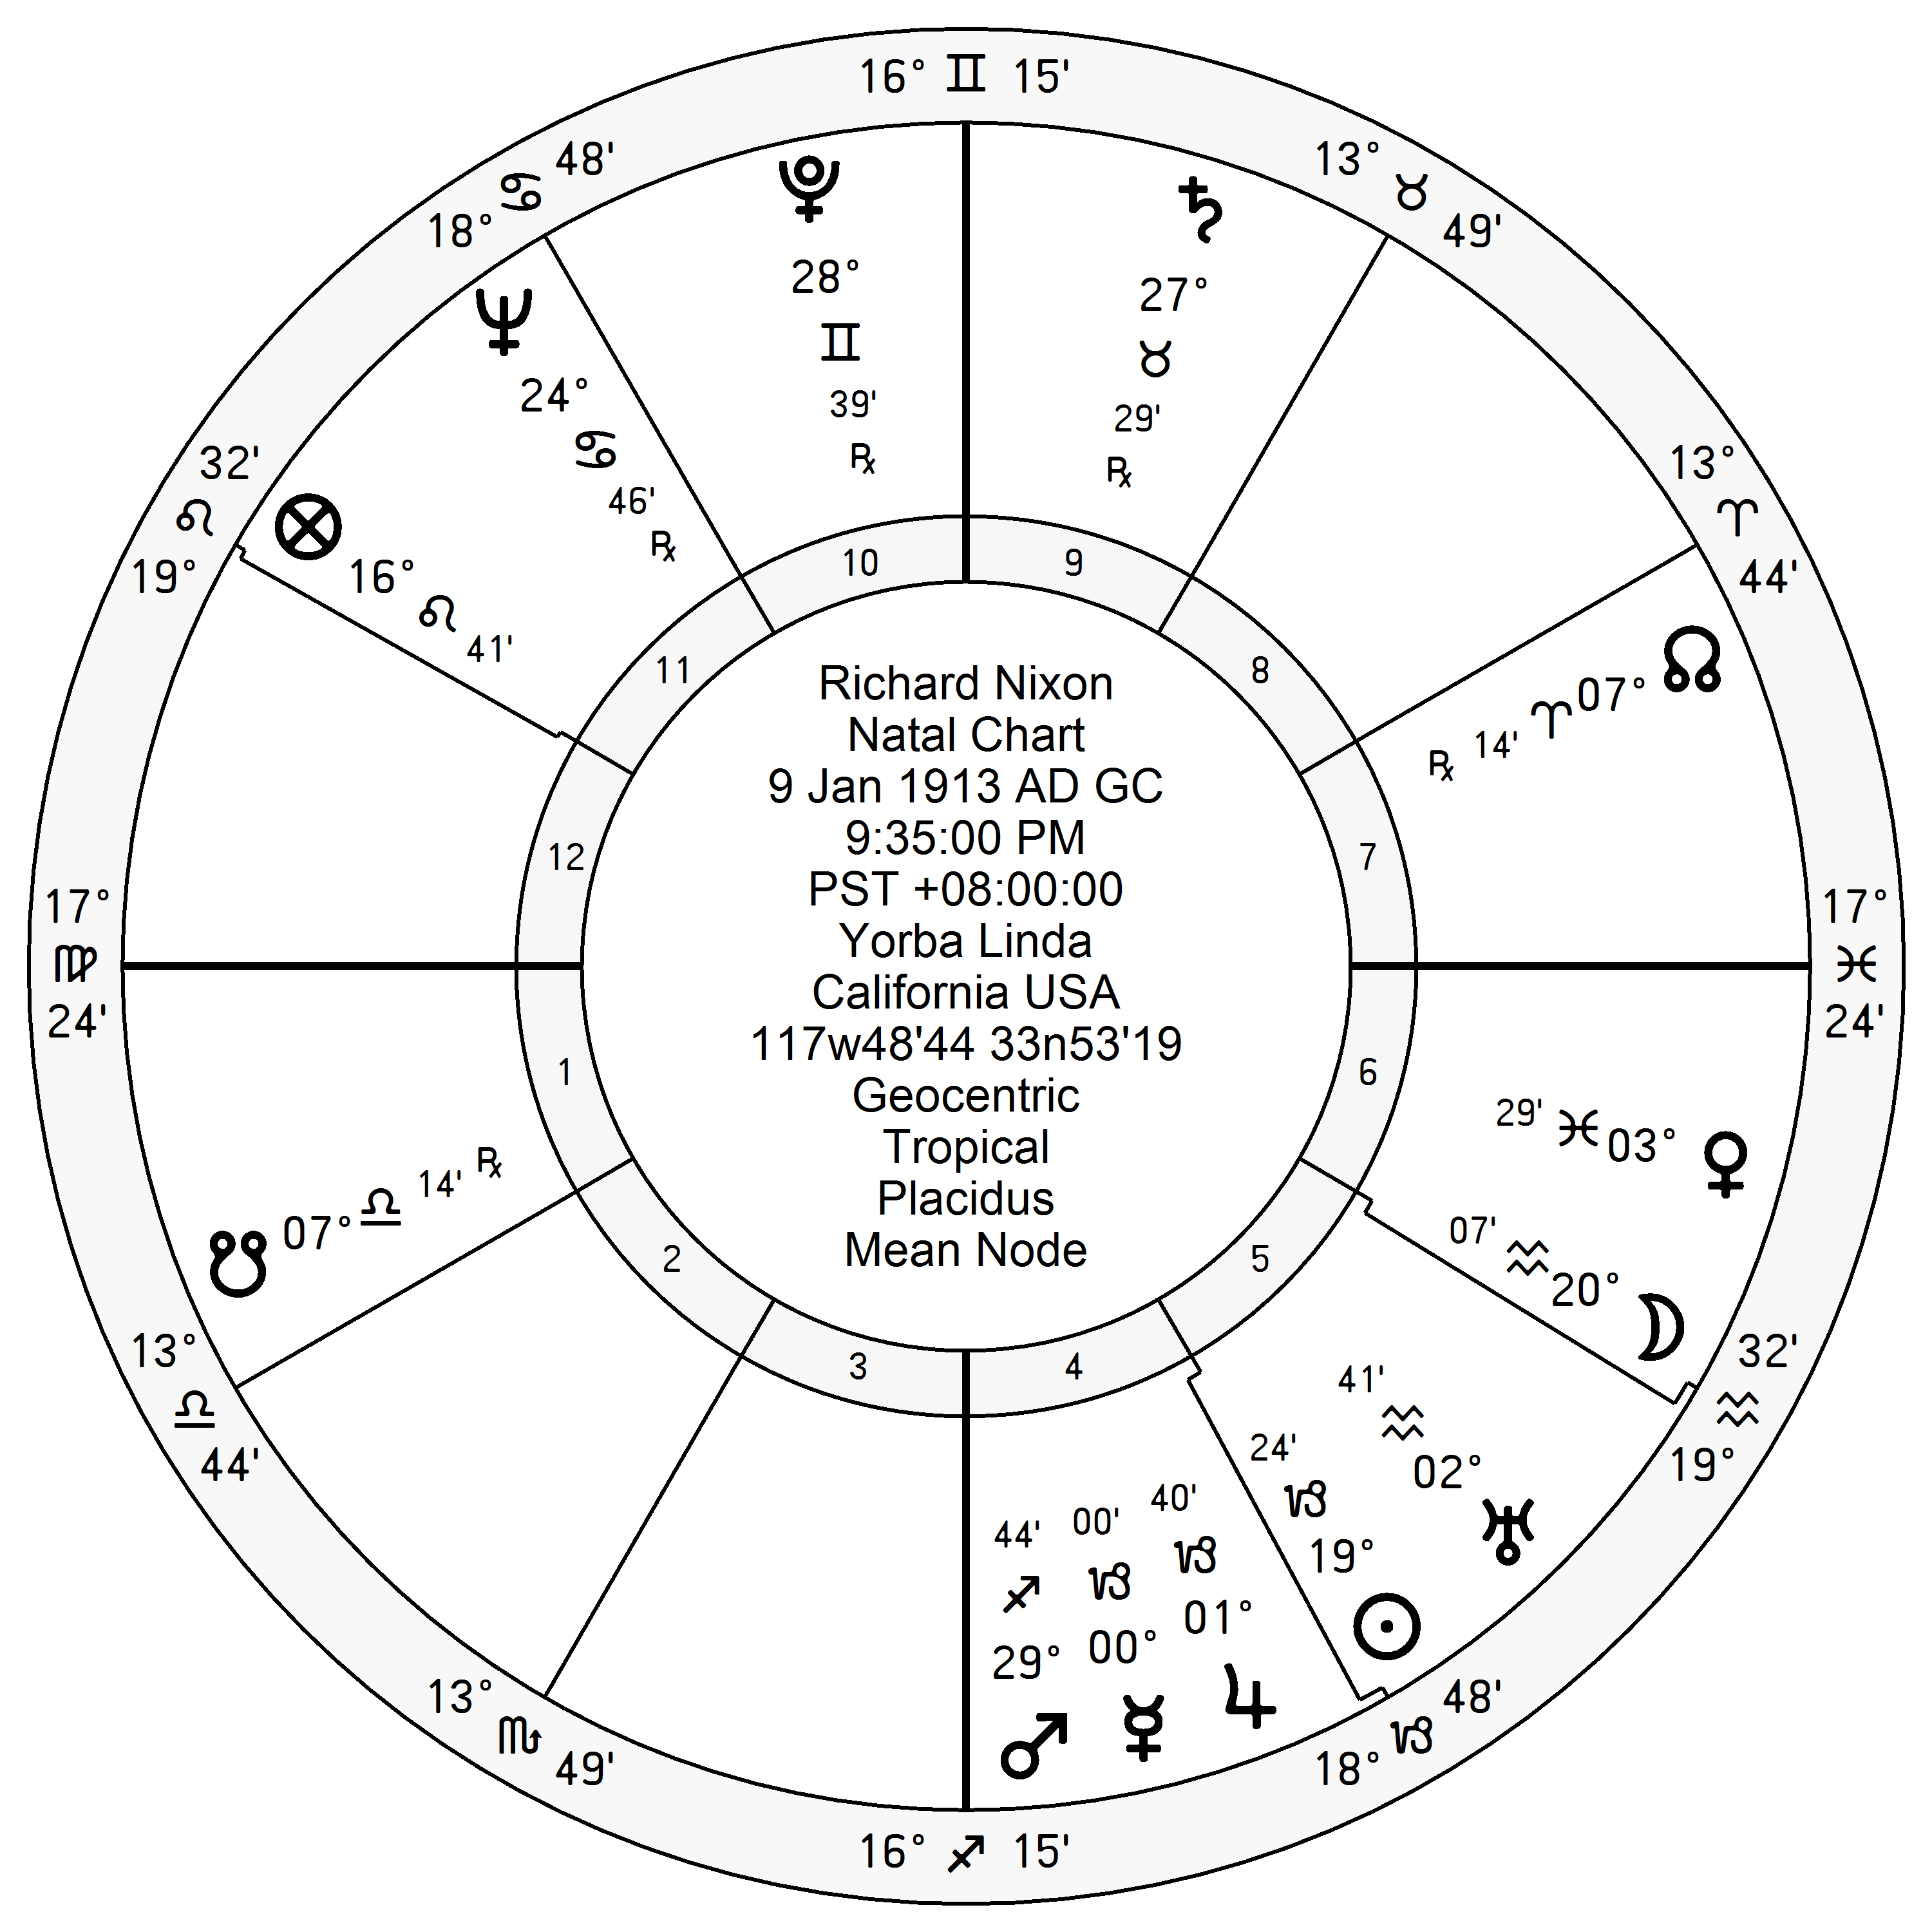
\includegraphics[width=0.9\textwidth]{charts/Nixon.png}}
\fontsize{8pt}{9pt}\selectfont

\Sun\, \Trine\, P10, \Trine\, N1 \\
\Venus\, \Square\, P10, \Opposition\, N1; \Trine\, N10 \\

The profection conditions are the same as those against JFK in 1960, only this time Nixon won.

\column{0.48\textwidth}
\vspace{-1em}
{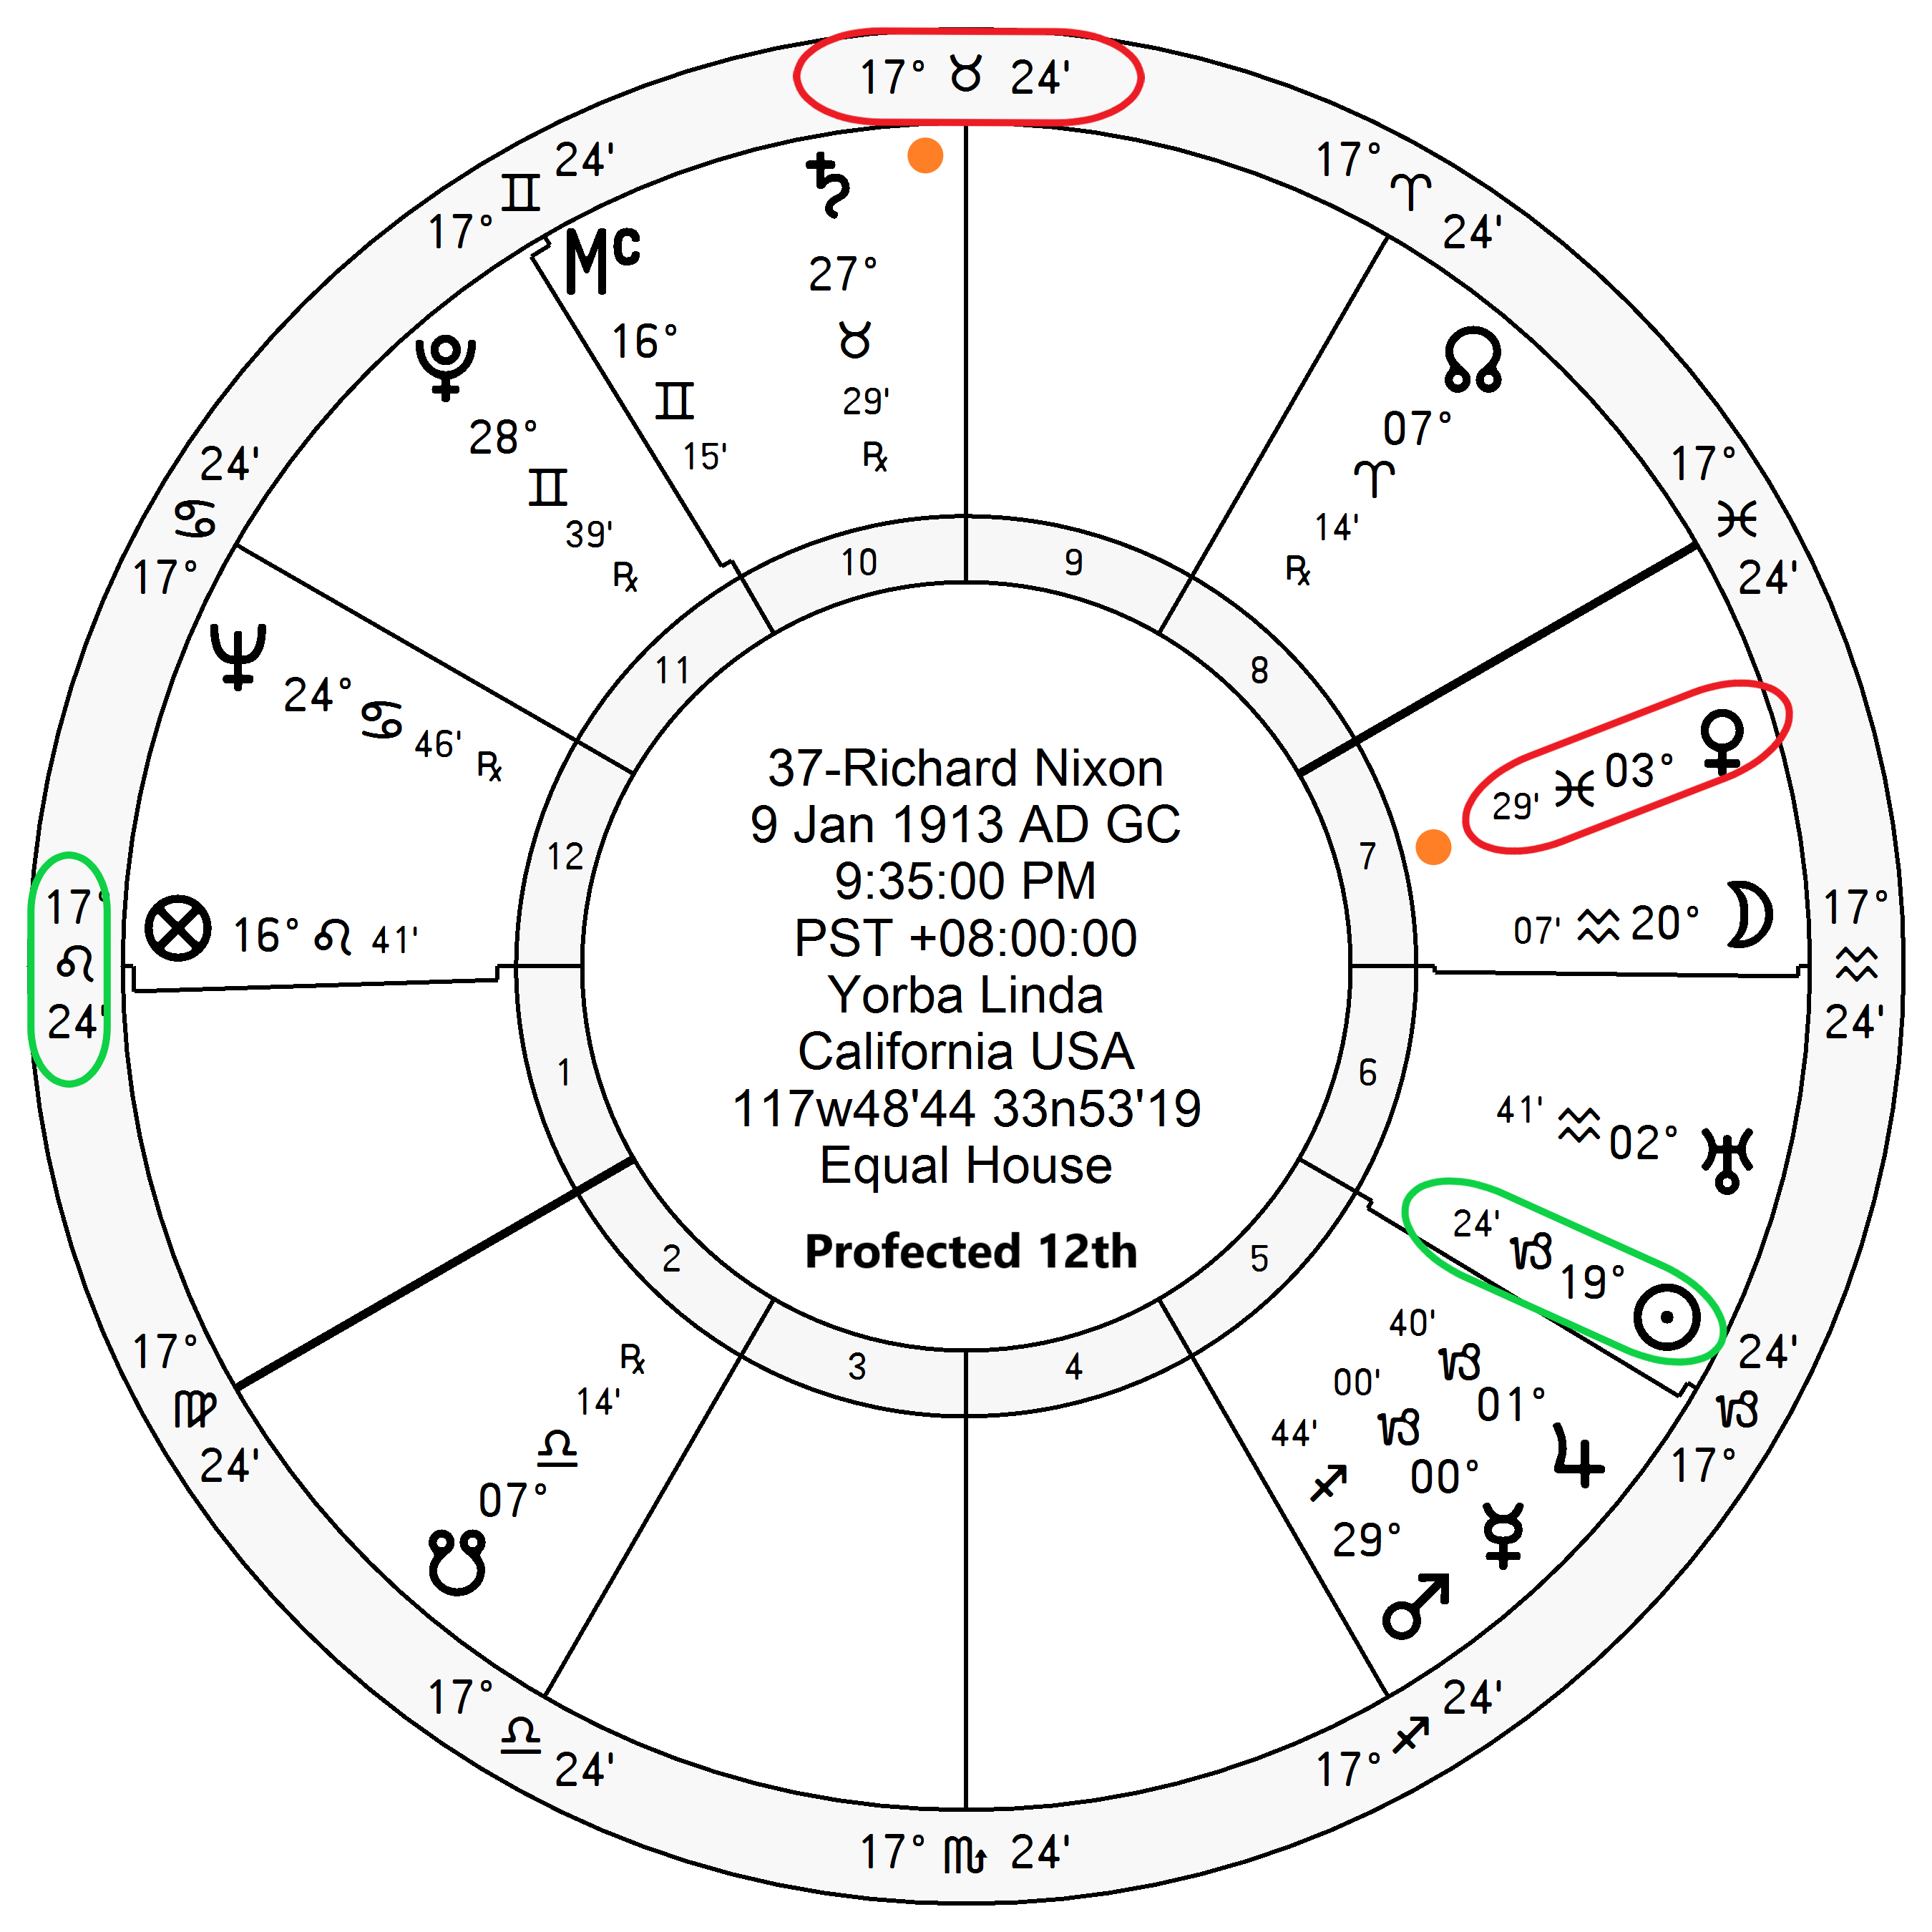
\includegraphics[width=0.9\textwidth]{charts/Nixon-Prof-12th.png}}
\fontsize{8pt}{9pt}\selectfont

\textbf{\dgreen P1=N12} 
	$\Rightarrow$ \Sun\, $\Rightarrow$ \textbf{\dgreen P6}/N5\\
\textbf{\red P10=N9}
	$\Rightarrow$ \Venus\, $\Rightarrow$ \textbf{\dgreen P7/N6}\\
PE=\textbf{\red P10/N9}
	 $\Rightarrow$ \Venus\, $\Rightarrow$ \textbf{\dgreen P7/N6}


\end{columns}
\end{frame}

% ===================================================
\begin{frame}[t]{Election November 7, 1972: George McGovern}
\small
\begin{columns}[T, onlytextwidth]
\column{0.48\textwidth}
\vspace{-1em}
{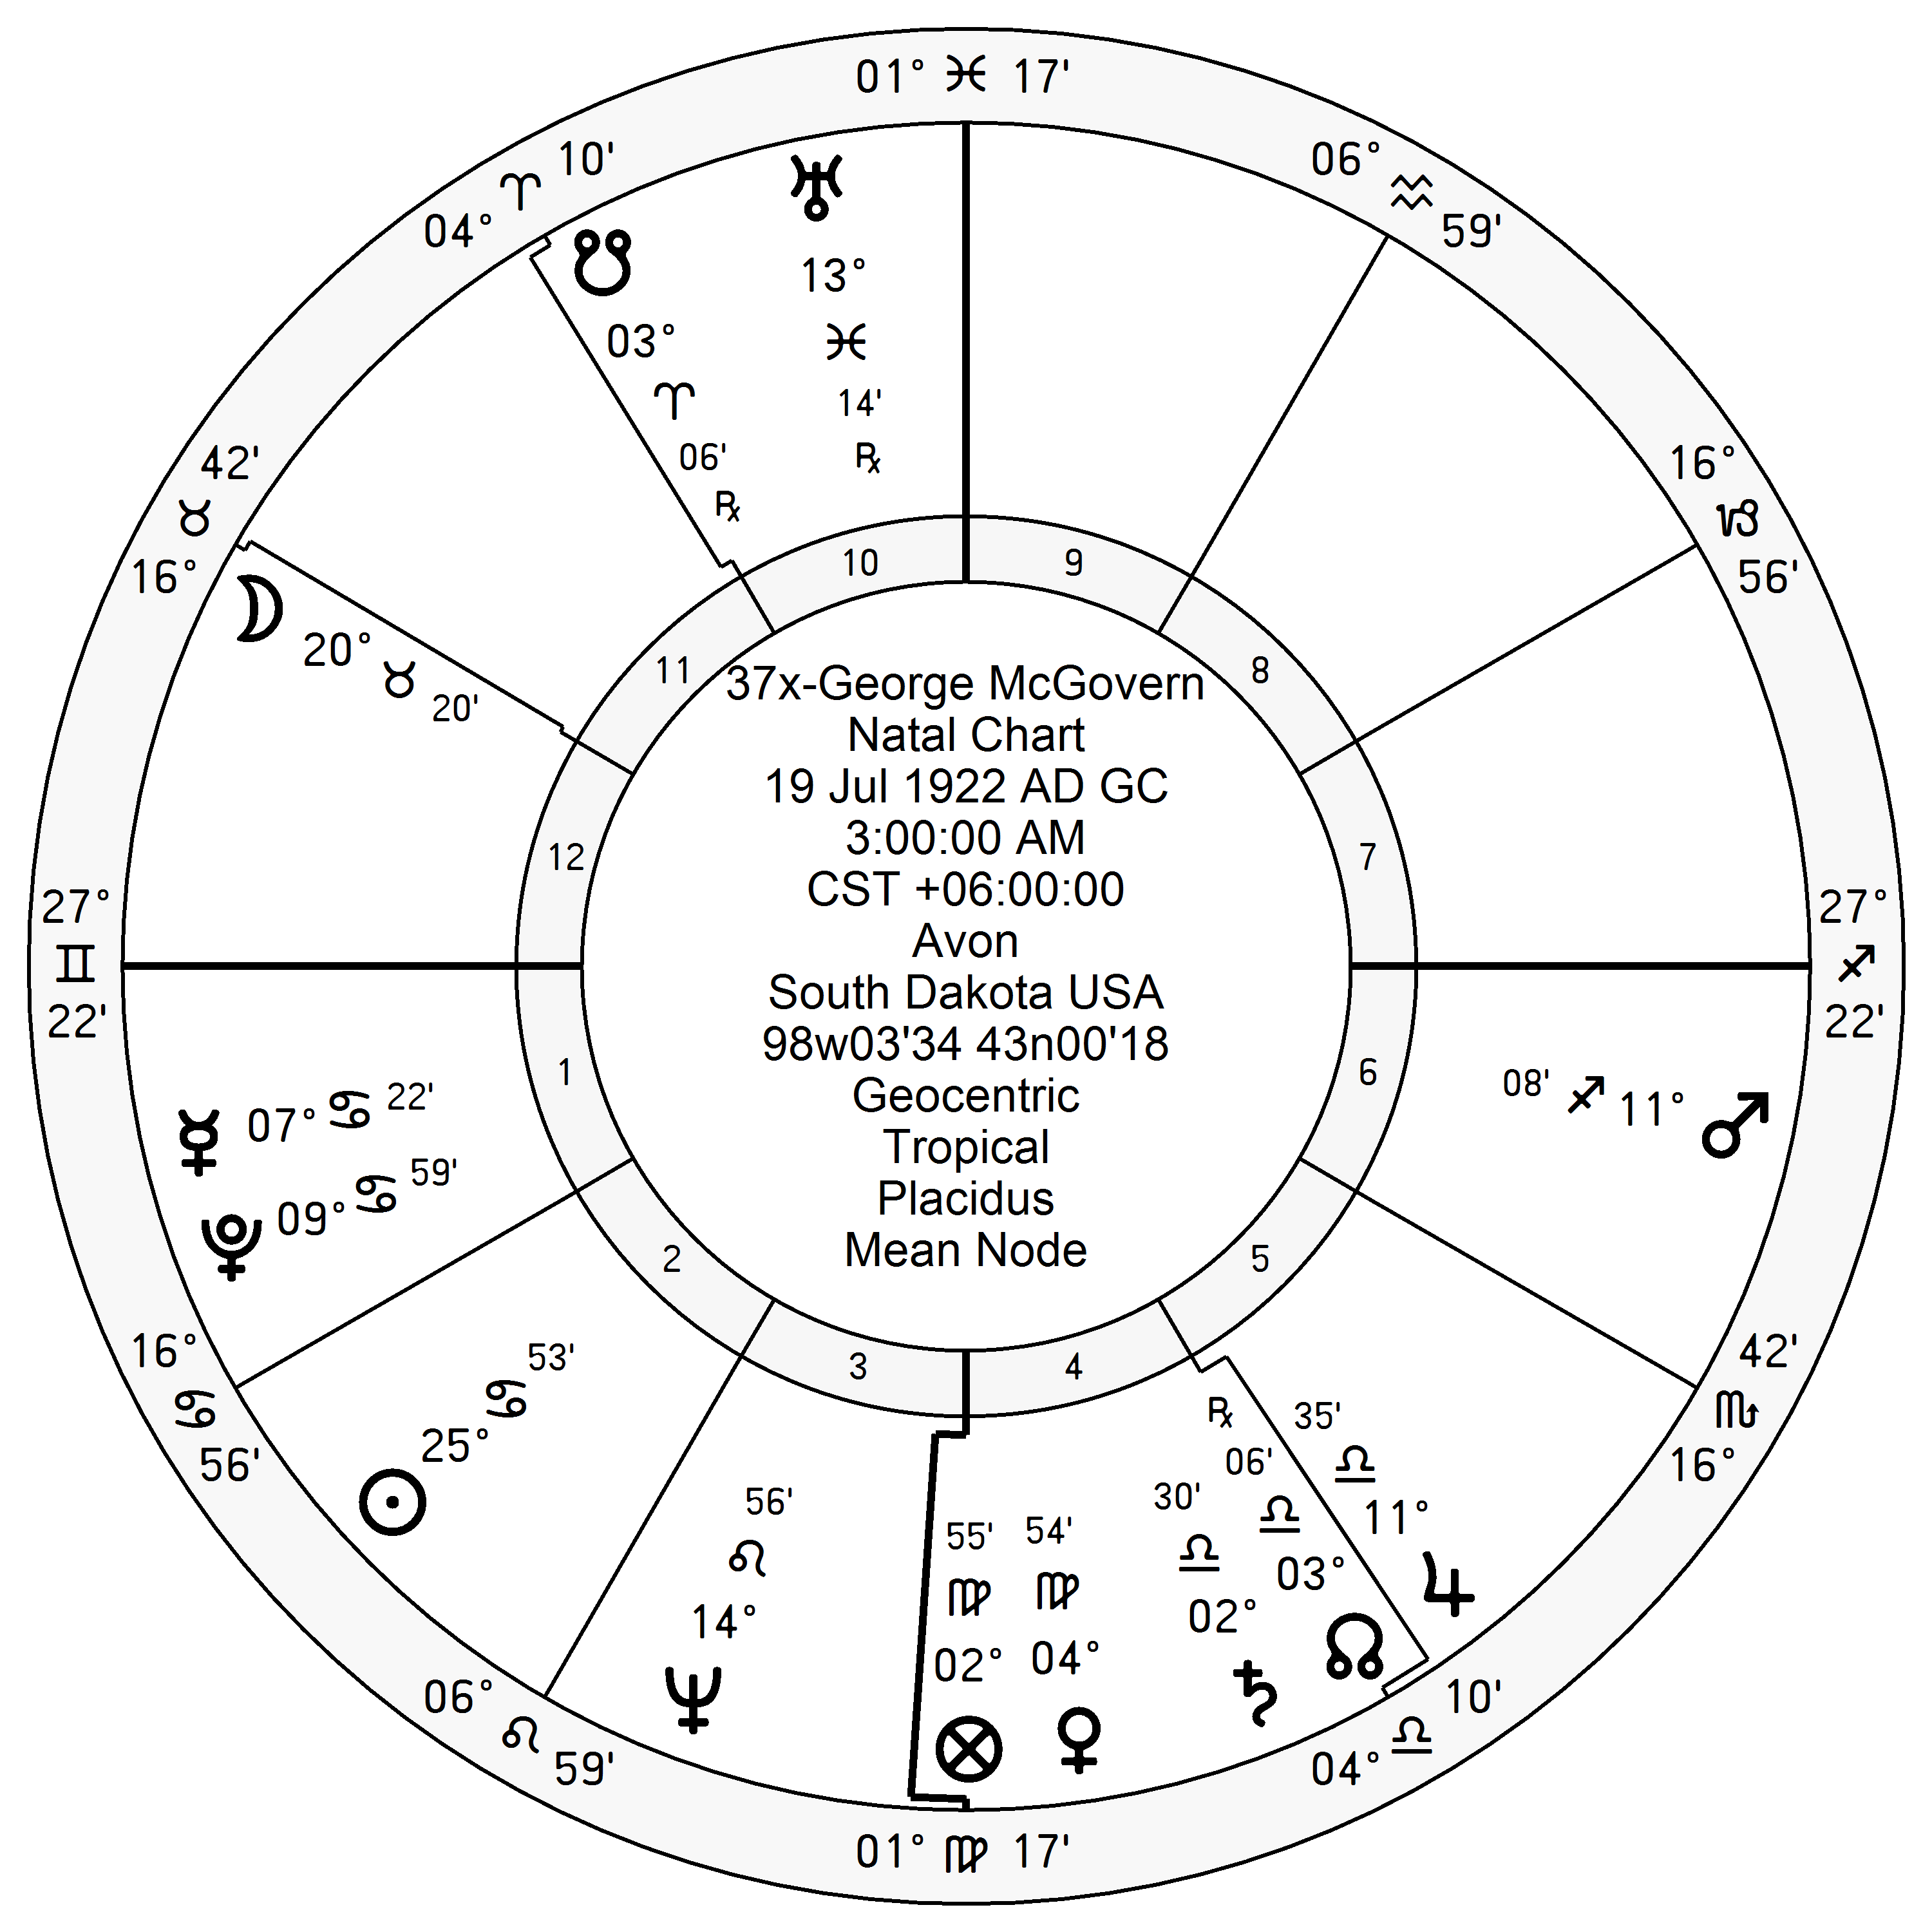
\includegraphics[width=0.9\textwidth]{charts/McGovern.png}}
\fontsize{8pt}{9pt}\selectfont

\Sun\, \Trine\, N10 \\
\Venus\, in P1, \Sextile\, N1; \Square\, P10, \Opposition\, N10 \\
\Mars\, \Opposition\, P10, \Square\, P1; \Square\, N10 \\
\vspace{0.5em}
The chart looks stronger than Nixon; \SouthNode\, in N10 weakens 10th? \Mars\, \Square\, \Venus?

\column{0.48\textwidth}
\vspace{-1em}
{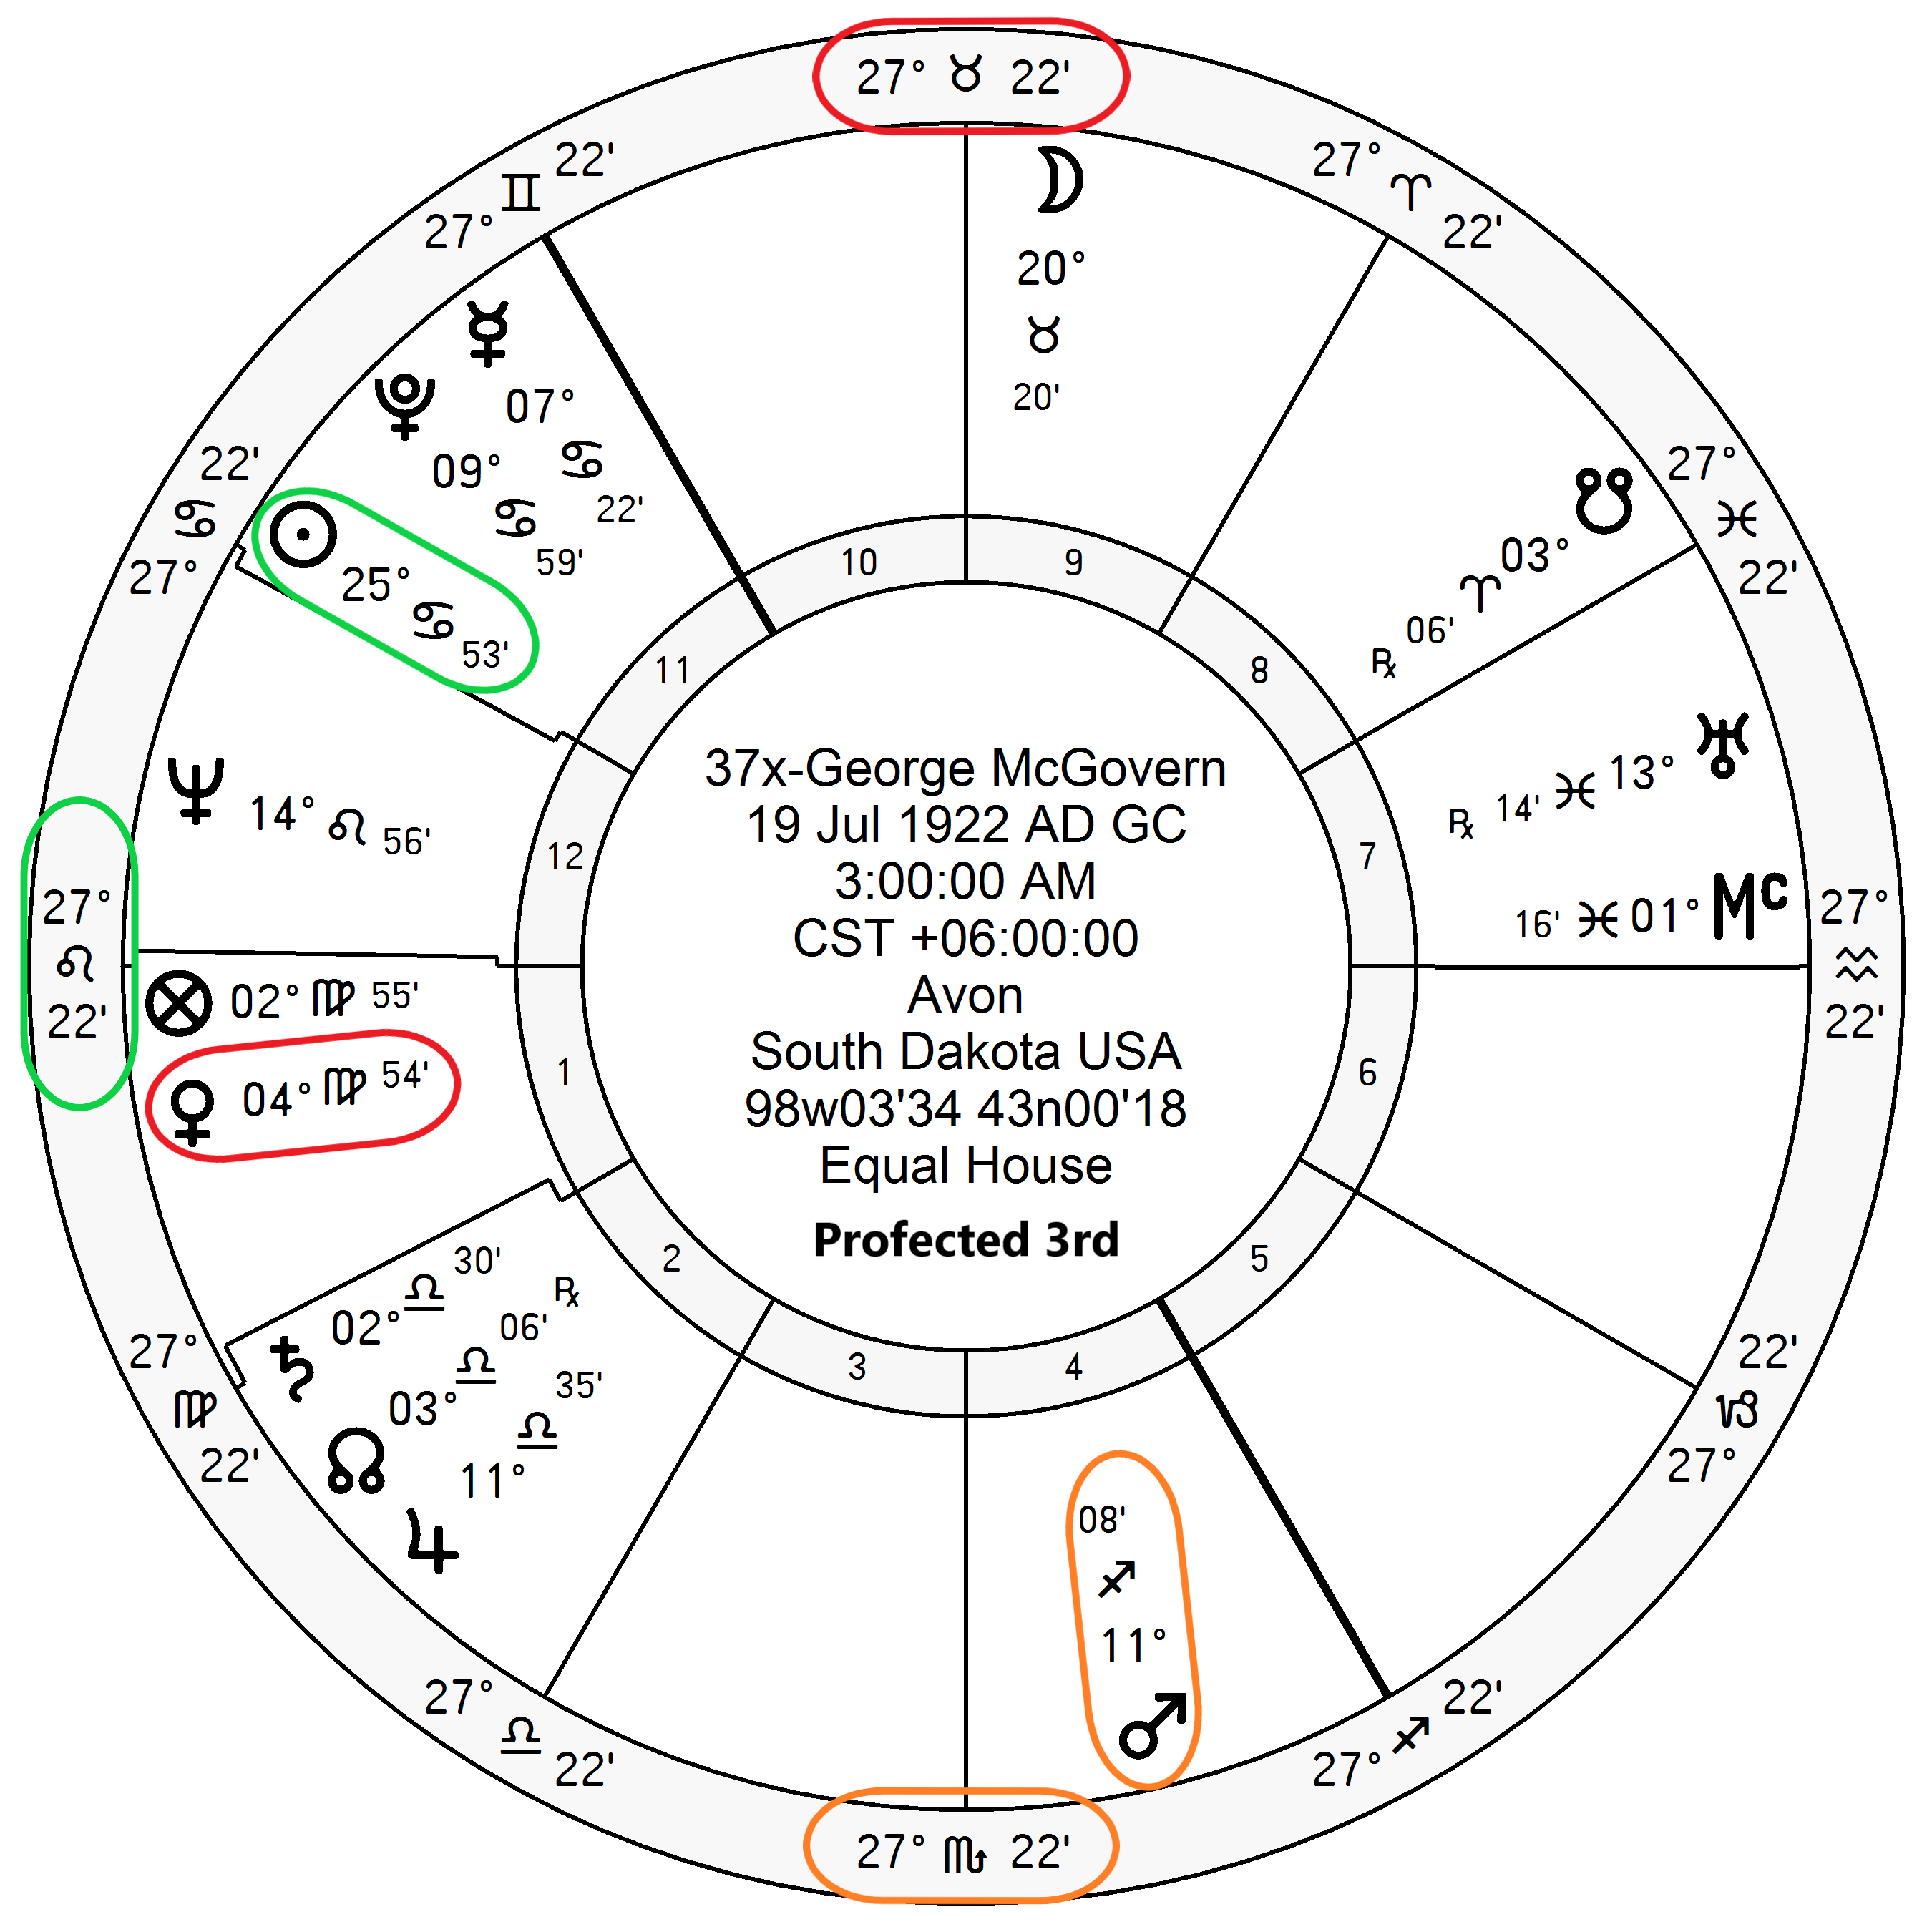
\includegraphics[width=0.9\textwidth]{charts/McGovern-Prof-3rd.png}}
\fontsize{8pt}{9pt}\selectfont
\textbf{\dgreen P1}=N3
	$\Rightarrow$ \Sun\, $\Rightarrow$ P11/N2\\
\textbf{\red P10=N12}
	$\Rightarrow$ \Venus\, $\Rightarrow$ \textbf{\dgreen P1}/\textbf{\red N4}\\
PE=\textbf{\red P4/N6}
	 $\Rightarrow$ \Mars\, $\Rightarrow$ \textbf{\red P4/N6}

\end{columns}
\end{frame}
